% !TEX root = ../main.tex

%\section{Properties of \kSum~and \zkclique~Hypotheses}
%\label{sec:kcliqueksumAllTHeThings}
In this section, we will prove the properties that \kSum~and \zkclique~have that will make them useful in constructing fine-grained OWFs and our fine-grained key exchange.

\subsection{\kSum~is Plantable from a Weak Hypothesis}
Here we will show that by assuming the Weak \kSum~hypothesis (see definition \ref{def:weak-k-sum}), we get that \kSum~is plantable and $n^{2+\delta}$-\ACIH. The proof is relatively straightforward: just show that planting a solution in a random \kSum-$R$ instance is easy while making sure that the distributions are close to what you expect.

\begin{theorem}
	Assuming the weak \kSum-$R$ hypothesis, \kSum-$R$ is plantable with error $\leq 2n^k/R$ in $O(n)$ time.
	%If the weak $k$-sum hypothesis holds over a range $R > 100 n^k$, then \kSum-$R$ is $n^{2+\delta}$-\ACIH.
	\label{thm:ksumPlantable}
\end{theorem}
\begin{proof}
	First, we will define $\Generate(n,b)$:
	\begin{itemize}
		\item $b = 0$: choose all $kn$ entries uniformly at random from $[0,R-1]$, taking time $O(n)$.
		\item $b = 1$: choose all $kn$ entries uniformly at random from $[0,R-1]$, then choose values $v_1, \dots, v_k$, each $v_i$ at random from partition $P_i$, and choose $i \getsr [k]$. Set $v_i = - \sum_{j \neq i} v_j \mod R$. This takes time $O(n)$.
	\end{itemize}
	
	We need to show that $\Generate(n,0)$ is $\epsilon$-close to $D_0$ and $\Generate(n,1)$ is $\epsilon$-close to $D_1$.
	
	First, we note that $\Generate(n,0)$ has the following property: $\Pr_{I \sim \Generate(n,0)}[I = I' | I\mbox{ has no solutions} ] = \Pr_{I \sim D_0}[I = I']$. This is because $\Generate(n,0)$ samples uniformly over the support of $D_0$. So, the total variation distance between $\Generate(n,0)$ and $D_0$ is the probability $\Generate(n,0)$ samples outside of the support of $D_0$, that is, the probability $\Generate(n,0)$ samples an $I$ with a value $1$ or greater. Let $\TVD$ denote Total Variation Distance between two distributions. Now, a union bound gives us
	\begin{align*}
	\TVD(\Generate(n,0), D_0) &= \Pr_{I \sim \Generate(n,0)}[I \mbox{ has at least 1 solution} ]\\ 
	&\le \sum_{\mbox{all $n^k$ sums $\vec s \in [n]^k$}} \Pr_{I \sim \Generate(n,0)}[\mbox{$\vec s$ is a \kSum}]\\
	&= \frac{n^k}{R}.
	\end{align*}
	
	Now, to show that $\Generate(n,1)$ is $\epsilon$-close to $D_1$, we will use the fact that total-variation distance ($\TVD$) is a metric and the triangle inequality. Let $\Generate(n,0) +$ Plant and $D_0 + $ Plant denote sampling from the first distribution and planting a \kSum~solution at random (so $\Generate(n,0) +$ Plant $= \Generate(n,1)$). We have that
	\begin{align*}
	\TVD(\Generate(n,1), D_1) &\le \TVD(\Generate(n,0) + \mbox{Plant}, D_0 + \mbox{Plant})\\
	&\qquad + \TVD(D_0 + \mbox{Plant}, D_1).
	\end{align*}
	The distance $\Generate(n,0) +$ Plant from $D_0 + $ Plant is equal to the distance from $\Generate(n,0)$ and $D_0$, since the planting does not change between distributions. As previously shown, this distance is at most $\frac{n^k}{R}$. The distance from $D_0 +$ Plant and $D_1$ is just the chance that we introduce more than one clique by planting. We are only changing one value in the $D_0$ instance, $v_i$. There are $n^{k-1} - 1 \le n^{k-1}$ possible sums involving $v_i$, so the chance that we accidentally introduce an unintended \kSum~solution is at most $\frac{n^{k-1}}{R}$. Therefore,
	\[\TVD(\Generate(n,1), D_1) \le \frac{n^k}{R} + \frac{n^{k-1}}{R} < \frac{2n^k}{R}\] \qed
\end{proof}

Note that when $R > 6n^k$, $\Generate(n,1)$ has total variation distance $< 1/3$ from $D_1(k-$SUM$-R,n)$.

\subsection{\zkclique~is also Plantable from Weak or Strong Hypotheses}
The proof in this section mirrors of the proof that \kSum-$R$ is plantable. Note that the size of a $k$-Clique instance is $O(n^2)$, and so the fact that this requires $O(n^2)$ time is just that it is linear in the input size. Here we will just list what the $\Generate$ functionality is:
\begin{itemize}
	\item $\Generate(n,0)$ outputs a complete $k$-partite graph with $n$ nodes in each partition, and edge weights drawn uniformly from $\Z_R$. This takes $O(n^2)$ time.
	\item $\Generate(n,1)$ starts with $\Generate(n,0)$, and then plants a clique by choosing a node from each partition, $v_1 \in P_1, \dots, v_k \in P_k$, choosing an $i \neq j \getsr [k]$, and setting the weight $w(v_i, v_j) = -\sum_{(i', j') \neq (i,j)} w(v_{i'}, v_{j'}) \mod R$. This also takes $O(n^2)$ time.\\
	If assuming the strong hypothesis (search problem), we can also output a witness, $(v_1,\ldots, v_k)$, of size $O(\log n)$.
\end{itemize}

Unfortunately for it seems difficult to show that \kSum~is average-case list-hard or splittable. However, we will show that if we assume that \zkclique~is only \emph{search} hard (a strictly weaker assumption than being indistinguishably hard), we can get the plantable, list-hard, and splittable properties --- the caveat is that we need to assume that \zkclique~requires $\~\Omega(n^k)$ time to solve (not just super-linear in time).

Before proving the theorem, we need a couple of helper lemmas to characterize the total variation distance, etc. These lemmas will be useful later on as well.

\begin{lemma}
	The distribution $D^{zkc}_{0}[R,n]$ has total variation distance $\leq n^k/R$ from the distribution of instances drawn from $\Generate(n,0)$.
	\label{lem:TVDnosol}
\end{lemma}
\begin{proof}	
	$D^{zkc}_{0}[R,n]$ is uniform over all instances of size $n$ where there are no solutions. $\Generate(n,0)$ is uniform over all instances of size $n$. 
	
	Let $D$ be the distribution of instances in $\Generate(n,0)$ which are in the support of $D^{zkc}_{0}[R,n]$. Because both $\Generate(n,0)$ and $D^{zkc}_{0}[R,n]$ are uniform over the support of $D^{zkc}_{0}[R,n]$, $D = D^{zkc}_{0}[R,n]$.
	
	So the total variation distance between $D^{zkc}_{0}[R,n]$ and $\Generate(n,0)$ is just 
	$$Pr_{I \sim \Generate(n,0)}[I \nin \text{ the support of } D^{zkc}_{0}[R,n]].$$
	
	The expected number of zero $k$-cliques is $n^k/R$, every set of $k$ nodes has a chance of $1/R$ of being a zero $k$-clique. Thus, the probability that an instance has a non-zero number of solutions is $\leq n^k/R$. So, the total variation distance is $\leq n^k/R$.
\end{proof}

\begin{lemma}
	The distribution $D^{zkc}_{1}[R,n]$ has total variation distance $\leq n^k/R+n^{k-2}/R$ from the distribution of $\Generate(n,1)$.
	\label{lem:TVDonesol}
\end{lemma}
\begin{proof}
	We want to first show that $\Generate(n,1)$ is uniform over the support of $D^{zkc}_{1}[R,n]$. Consider an instance $I$ in the support of $D^{zkc}_{1}[R,n]$. Let $S(I) = {a_1, \ldots , a_k}$ be the set of $k$ nodes in which there is a zero $k$-clique. $Pr_{I' \sim \Generate(n,1)}[I' = I]$ is given by the chance that
	\begin{itemize}
		\item the nodes chosen in $I'$ ($a_1',\ldots, a_k'$) to plant a clique are the same as those in $S(I)$,
		\item the edges in the clique have the same weights in $I'$ and $I$ and,
		\item all edges outside the clique have the same weight in $I'$ and $I$. 
	\end{itemize}
	$$Pr_{I' \sim \Generate(n,1)}[I' = I] = \left(n^{-k} \right)  \left(R^{-\binom{k}{2}-1} \right)  \left(R^{-\binom{k}{2}(n^2-1)} \right) .$$
	
	This is the same probability for all instances $I$ in the support of $D^{zkc}_{1}[R,n]$. 
	
	So, we need only bound the probability 
	$$Pr_{I \sim \Generate(n,1)}[I \nin \text{ the support of } D^{zkc}_{1}[R,n]].$$
	
	By Lemma \ref{lem:TVDnosol} the initial process of choosing edges the probability of producing a clique is $\leq n^k/R$. We then change one edge's weight, this introduces a clique. It introduces an expected number of additional cliques $\leq n^{k-2}/R$ (this is the number of cliques it participates in). Thus, we can bound the probability of more than one clique by $\leq n^k/R+n^{k-2}/R$.
\end{proof}



\begin{theorem}\label{thm:zkcPlantable}
	Assuming the weak \zkclique~hypothesis (\ACIH) over range $R$, \zkclique~is $(O(n^2), 2n^k/R)$-Plantable.\\
	Assuming the strong \zkclique~hypothesis (\ACSH) over range $R$, \zkclique~is also $(O(n^2), 2n^k/R)$-Plantable.
\end{theorem}
\begin{proof}
	This proof simply combines the two previous lemmas: Lemma \ref{lem:TVDnosol} and Lemma \ref{lem:TVDonesol}.
	
	$\Generate(n,0)$ has total variation distance $n^k/R$ from $D^{zkc}_{0}[R,n]$ by Lemma \ref{lem:TVDnosol}, and $\Generate(n,1)$ has total variation distance $n^k/R+n^{k-2}/R < 2n^k/R$ from $D^{zkc}_1[R,n]$ by Lemma \ref{lem:TVDonesol}. So, in both cases the error is bounded above by $2n^k/R$.
	
	
	
	Finally note that $\Generate(n,1)$ also can output the planted solution, the clique it chose to set to 0, and so can output a witness.
\end{proof}


\subsection{\zkclique~is Plantable, Average Case List-Hard and, Splittable from the Strong \zkclique~Hypothesis}
\label{sec:zkcIsAllTheThings}

Here we will focus on the Strong \zkclique~assumption, see Definition \ref{def:strongzkc}. Recall that this is the search version of the problem: given a graph with weights on its edges drawn uniformly from the $k$-partite graphs with exactly one zero $k$-clique, it is difficult to find the clique in time less than $\~O(n^k)$.

We already proved that \zkclique~was Plantable in Theorem \ref{thm:ksumPlantable}. So, now we will focus on the other two properties we want: list-hardness and splittability. These will give us the properties we need for our key exchange.

%There are two main differences from the notion of plantable in this case and in the previous section. First, our strong hypothesis is actually a \emph{search problem}, and unfortunately, there is no average-case to average-case reduction from search to decision for \zkclique~that we are aware of. The existing worst-case reductions break down because of the need for recursion and the error we allow our adversary\footnote{The recurrence really throws us for a loop, so to speak.}. The second difference is the strength of the assumption: we require a large gap between how fast honest parties can plant and how long it takes for an adversary to find a solution in a planted instance. That is, the while we take $O(n^2)$ time to plant a solution, we assume an adversary must take $O(n^k)$ time to find the solution (instead of just $O(n^{2(1 + \delta)})$).

%Now we will prove that \zkclique~has the properties we need for our key exchange. 

%\subsubsection{\zkclique~is a Plantable Problem}
%
%The proof of this theorem follows from the proof for theorem \ref{thm:zkcPlantable}, even though it was for the decision version of Plantability.
%\begin{theorem}
%	Assuming the weak \zkclique~hypothesis over range $R$, \zkclique~is plantable with error $\leq 2n^k/R$ in $O(n^2)$ time.
%\end{theorem}
%%The idea is that $\Generate(n)$ is the same as $\Generate(n,1)$ for the decision version. We proved that $\Generate(n,1)$ has TVD from $D_1$ at most $2n^k/R$, which finishes the proof.
%\begin{proof}
%	The proof of this will mirror the proof that \kSum~is plantable. Note that the input size for \zkclique~is $O(n^2)$ when there are $kn$ nodes, unlike the input size for \kSum~(which is $O(n)$). We define $\Generate$ as follows:
%	\begin{itemize}
%		\item $\Generate(n,0)$ outputs a complete $k$-partite graph with $n$ nodes in each partition, and edge weights drawn uniformly from $\Z_R$. This takes $O(n^2)$ time.
%		\item $\Generate(n,1)$ starts with $\Generate(n,0)$, and then plants a clique by choosing a node from each partition, $v_1 \in P_1, \dots, v_k \in P_k$, choosing an $i \neq j \getsr [k]$, and setting the weight $w(v_i, v_j) = -\sum_{(i', j') \neq (i,j)} w(v_{i'}, v_{j'}) \mod R$. This also takes $O(n^2)$ time.
%	\end{itemize}
%	Showing $\Generate(n,0)$ has TVD at most $n^k/R$ from $D_0$ for the same reason as \kSum: $\Generate(n,0)$ is uniform over the support of $D_0$ (just like $D_0)$, and so the distance is equal to the probability $\Generate(n,0)$ produces an instance with one or more zero $k$-cliques. There are $n^k$ different possible cliques and a union bound yields the probability that one of them has weight zero is simply $n^k/R$.
%	
%	Then showing $\Generate(n,1)$ has TVD at most $n^k / R + n^{k-2}/R$ from $D_1$ is just as before: $TVD(\Generate(n,1), D_1) \le TVD(\Generate(n,0) + \mbox{Plant}, D_0 + \mbox{Plant}) + TVD(D_0 + \mbox{Plant}, D_1)$. The first term is just $TVD(\Generate(n,0), D_0) \le n^k/R$. The second is just the probability that Plant introduces an unintended zero-clique. Since we are only changing one edge when we plant, the probability that this happens is at most $(n^{k-2} - 1)/R \le n^{k-2}/R$; that changed edge fixes two out of the $k$ edges we choose, and so there are $k-2$ partitions left to choose from.
%	
%	Therefore, in total, the error from $\Generate$ is at most $2n^k/R$.
%	\qed
%\end{proof}



\subsubsection{\zkclique~is Average Case List-Hard}

%Also true for the decision version! If we want the decision version instead 
% We can include the commented out points about D_0
We present the proof that \zkclique~is average case list-hard.

The intuition of the proof is as follows. There is an efficient worst case self-reduction for the \zkclique~problem. This self-reduction results in $\ell'(n)^k$ subproblems of size $n/\ell'(n)$. One can choose $\ell'(n)$ of these instances such that they are generated from non-overlapping parts of the original instance. They will then look uniformly randomly generated. 

Now we will have generated many, $(\ell'(n))^k$, of these list versions of the \zkclique~ problem, where only one of them has the unique solution. We show that the problem is Average Case List-Hard by demonstrating that we can make many independent calls to the algorithm despite correlations between the instances called. Specifically, we only care about the response on one of these instances, so as long as that instance is random then we can solve the original problem. 


\begin{theorem}
	Given the \strongzkc, \zkclique~is Average Case List-Hard with list length $\ell(n)$ for any $\ell(n) = n^{\Omega(1)}$.
	\label{thm:zkcAvgListHard}
	%\label{thm:zkcSelfReduce}
\end{theorem}
\begin{proof}
	Let $\ell = \ell(n)$ for the sake of notation. $I \sim D_1(\mbox{\zkclique}, \ell \cdot n)$ with $k$ partitions, $P_1, \ldots, P_k$ of $\ell \cdot n$ nodes each and with edge weights generated uniformly at random from $\Z_R$.
	
	Randomly partition each $P_i$ into $\ell$ sets $P_i^1, \ldots, P_i^\ell$ where each set contains $n$ nodes. Now, note that if we look for a solution in all $\ell^k$ instances formed by taking every possible choice of $P_1^{i_1}, P_2^{i_2},\ldots, P_k^{i_k}$, this takes time $O((\ell\cdot  n)^k)$, which is how long the original size $\ell n$ problem takes to solve. 
	
	Sadly, not all $\ell^k$ instances are independent. We want to generate sets of independent instances. Note that if we choose $\ell$ of these sub-problems such that the nodes don't overlap, then the edges were chosen independently between each instance! Specifically consider all vectors of the form $\vec{x} = \langle x_2, \ldots, x_k\rangle \in \mathbb{Z}_{\ell}^{k-1}$. Then let 
	$$S_{\vec{x}}= \{P_1^i \cup P_2^{i+x_2} \cup \ldots \cup P_k^{i+x_k}|\forall i\in [1,\ell]\}$$
	be the set of all independent partitions. Now, note that $\cup_{\vec{x} \in \mathbb{Z}_\ell^{k-1}} S_{\vec{x}}$ is the full set of all possible $\ell^k$ subproblems, and the total number of problems in all $S_{\vec{x}}$ is $\ell^k$, so once again brute-forcing each $S_{\vec{x}}$ takes time $O((\ell \cdot n)^k)$. We depict this splitting in Figure \ref{fig:listHardReduction}.
	
	\begin{figure}[h]
		\centering
		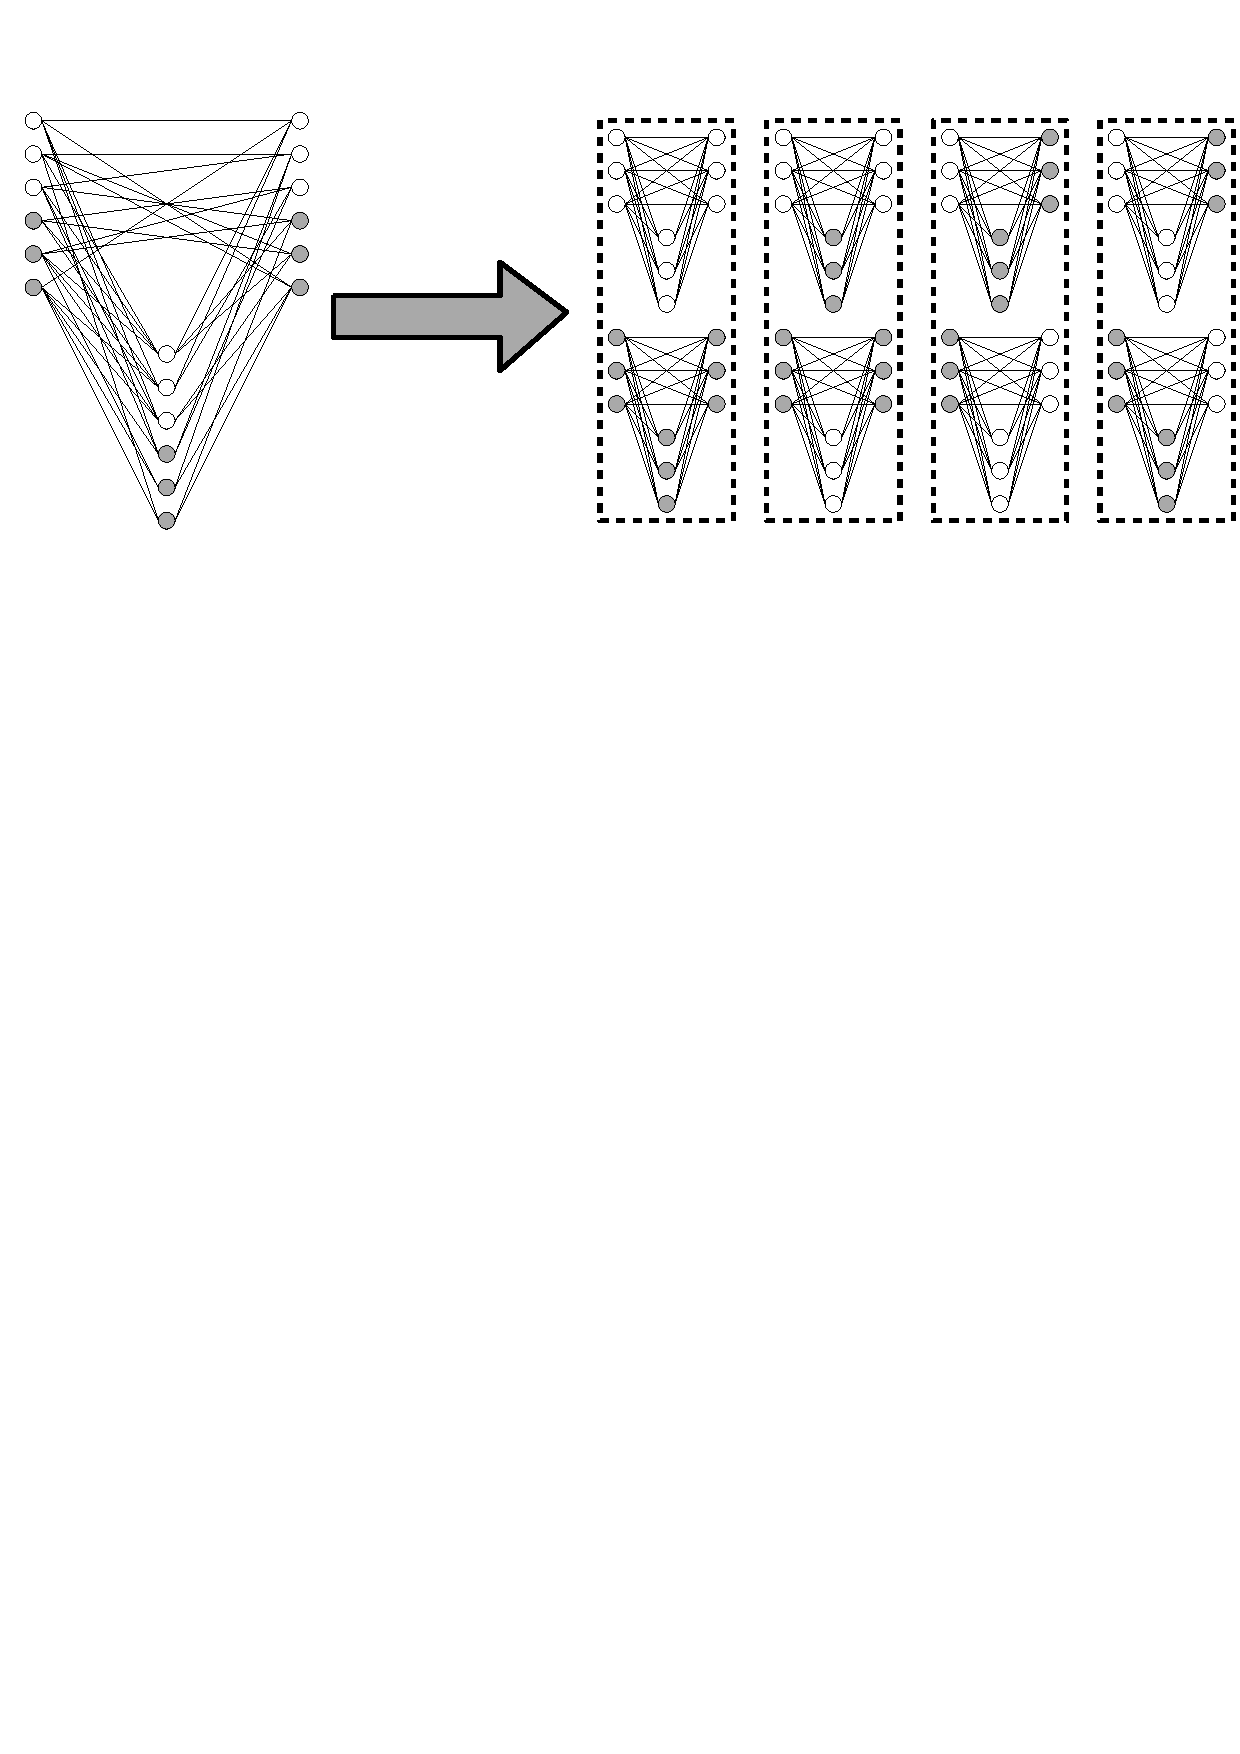
\includegraphics[scale=0.6]{fgcrypto/list-hard-fig.pdf}
		\caption{A depiction of splitting the subproblems for a case where $\ell=2$ and $k=3$.}
		\label{fig:listHardReduction}
	\end{figure}
	
	Note that producing these each of these $\ell$ instances is efficient, it takes time $O(n^2)$, which is just the input size.
	
	Next, we will show that the correct number of solutions are generated. 
	If $I$ has only one solution then exactly one $I_j$ in exactly one $S_{\vec{x}}$ has a solution. This is because any zero-$k$-clique in $I$ must involve exactly one node from each partition $P_i$. So, if there is one zero-$k$-clique it will only appear in subproblems where the node from partition $P_i$ is in  $P_i^j$ and $P^i_j$ appears in that subproblem. There is exactly one sub-problem generated with a specific choice of $k$ sub-partitions. So, exactly one $I_j$ in exactly one $S_{\vec{x}}$ has a solution.
	
	Let $S^*$ be the list $S_{\vec x}$ that contains a \zkclique. We have that the $S_{\vec{x}}$ which actually contains an instance with a solution is drawn from
	\[ \{I_1, \dots, I_x\}_{I_i \sim D_{1}, \land \forall j \neq i, I_j \sim D_{0}}.\]
	This distribution is exactly what we require for a list-problem. All that is left to show is if we have $\PFT{\ell \cdot n^k}$ adversary $\cA$ that can identify for which index $i$ there is a zero $k$-clique in $S^*$ (with probability at least 7/10), we can use $\cA$ to find the clique.
	
	%	By Lemma \ref{lem:TVDonesol} the original instance the distribution is within total variation distance of $n^k/R + n^{k-1}/R$ from planting a clique after uniformly at random picking the weight for each edge. 
	
	%	In the planted distribution, the instances in $S_{\vec{x}}$ which do not contain the planted clique have had their edges chosen uniformly at random. Thus, by Lemma \ref{lem:TVDnosol} they each have total variation distance $(n/g)^k/R$ from the distribution $D_{0}=D^{zkc}_{0}[R,n/g]$. 
	
	%	The instance which contains the planted solution itself had all edges chosen uniformly at random except for the planted clique edge. Thus, by Lemma \ref{lem:TVDonesol} it has total variation distance $(n/g)^k/R + (n/g)^{k-1}/R$ from $D_{1}= D^{zkc}_{1}[R,n/g]$. Which index within $S_{\vec{x}}$ this clique lands uniform over all the $g$ indices, because the clique nodes were picked uniformly at random. 
	
	%	The total error introduced by this process is $\leq g(n/g)^k/R+ (n/g)^{k-1}/R+n^k/R + n^{k-1}/R \leq 2n^k/R$ for $g>2$ and sufficiently large $n$. 
	%	
	%	We make no constraints on $g$ other than that $1<g<n$
	
	Now, recall that we are trying to solve a search problem: we need to be able to turn an index pointing to partitions into a witness for the original problem. According to the strong \zkclique~hypothesis, this search requires $O(n^k)$ time. However, as long as $\ell = n^{\Omega(1)}$, this is still faster in a fine-grained sense.
	
	On an input $I$ from $D_1$, algorithm $\cB$ uses $\cA$ as follows:
	\begin{itemize}
		\item Randomly partition each $P_i$ from $I$ into $\ell$ parts.
		\item For every $\vec x \in \Z_{\ell}^{k-1}$:
		\begin{itemize}
			\item Generate the list $S_{\vec x}$.
			\item Run $\cA(S_{\vec x})$ to get output $i$.
			\item Brute force search the size-$n^2$ \zkclique~instance $S_{\vec x}[i] = (P_1^i, \ldots, P_k^{i + x_k})$ for a solution. If one exists, output it, otherwise, continue.
		\end{itemize}
	\end{itemize}
	
	The first step only takes $O(\ell \cdot n)$ time since we are only divvying up $\ell n$ nodes. The second step requires a bit more analysis. The loop runs at most $\ell^{k-1}$ times. Each time the loop runs, it only takes $O(\ell \cdot n)$ time to construct $S_{\vec x}$, while $\cA$ takes $O((\ell \cdot n^{k})^{(1-\epsilon)})$ (since it is $\PFT{\ell \cdot n^k}$), and our brute force check takes $O(n^k)$ time. Putting this together, the algorithm takes a total time of 
	\[O(\ell \cdot n + \ell^{k-1} ((\ell \cdot n^{k})^{(1-\epsilon)} + n^k + \ell \cdot n) ) = O(\ell^{k-\epsilon}n^{k(1-\epsilon)} + \ell^{k-1}n^{k}) + \ell^k \cdot n.\]
	Both terms in this sum are strictly less than the hypothesized $\ell^k n^k$ time, and so $\cB$ is $\PFT{(\ell n)^k}$, contradicting the strong \zkclique~hypothesis.
	
	The reason we require $\ell(n) = n^{\Omega(1)}$ is because if it were less than polynomial in $n$, we would not get noticeable improvement through this method of splitting up the problem into several sub-problems --- the brute force step would take as long as solving the original problem via brute force.
	\qed
\end{proof}


\subsubsection{\zkclique~is Splittable}
Next we show that zero-k-clique is splittable. We start by proving this for a convenient range and then show we can use a reduction to get more arbitrary ranges. 

\paragraph{Splitting the problem over a convenient range.} Intuitively we will split the weights in half bit-wise, taking the first half of the bits of each edge weight, and then we take the second half of the bits of each edge weight to make another instance. If the $\binom{k}{2}$ weights on a $k$ clique sum to zero then the first half of all the weights sum to zero, up to carries, and the second half of all the weights sum to zero, also up to carries. We simply guess the carries. 

\newcommand{\high}[1]{{#1}^\uparrow}
\newcommand{\low}[1]{{#1}_\downarrow}
\newcommand{\ZkC}{\mathrm{Z}$k$\mathrm{C}}

\begin{lemma}
	\zkclique~is generalized splittable with error $\leq 4(\binom{k}{2} + 1) n^k/\sqrt{R}$ when $R=4^{x}$ for some integer $x$. 
	\label{lem:zkcSplitConvenientRange}
\end{lemma}
\begin{proof}
	We are given an instance of \zkclique~$I$ with $k$ partitions, $P_1, \ldots, P_k$ of $n$ nodes and with edge weights generated uniformly at random from $[0,R-1]$, where $R = 2^{2x}$ for some positive integer $x$.

	First we will define some helpful notation to describe our procedure.
	\begin{itemize}
		\item Let $\ZkC[R]$ denote the \zkclique~problem over range $R$.
		\item Let $w(P_i[a],P_j[b])$ be the weight of the edge in instance $I$ between the $a^{th}$ node in  $P_i$ and the $b^{th}$ node in $P_j$.
		\item Let $u$ be some number in the range $[0,R-1]$. Let $\high{u}$ be the high order $\lg(R)/2$ bits of the number $u$ (this will be an integer because $R$ is a power of 4). Let $\low {u}$ be the low order $\lg(R)/2$ bits of the number $u$.\\
		For the sake of notation, $\high w (P_i[a], P_j[b])$ denotes $\high{[w (P_i[a], P_j[b])]}$, and same for $\low w (P_i[a], P_j[b])$ denoting $\low {[w (P_i[a], P_j[b])]}$.
	\end{itemize}

	\newcommand{\lowI}{I_{low}}
	\newcommand{\highI}{I_{high}}
	Here is the reduction to take one instance of $\ZkC[R]$ and create a list of pairs of instances of $\ZkC[\sqrt R]$.
	%TODO: should put this in an algorithm
	\begin{enumerate}
		\item Take the $\ZkC[R]$ instance $I$ and create two instances of $\ZkC[\sqrt R]$, $\lowI$ and $\highI$ by the following:
		\begin{itemize}
			\item For every edge $(P_i[a], P_j[b])$ in $I$, let the corresponding edge in $\lowI$ have weight $\low w(P_i[a], P_j[b])$ and the edge in $\highI$ have weight $\high w(P_i[a], P_j[b])$.
		\end{itemize}
		\item For every $c \in [0,\binom k 2]$ (we need only check $\binom k 2$ possible carries):% because we are summing $\binom k 2$ numbers each of which are less than $1$):
		\begin{enumerate}
			\item Let $I_1^{c}$ be a copy of $\lowI$, but randomly permute all nodes.
			\item Let $I_2^{c}$ be a copy of $\highI$, but choose a random pair of a partitions $P_i$ and $P_j$: for all edges $e_2 \in I_2^{c}$ between $P_i$ and $P_j$, a copy of edge $e \in \highI$, let $w(e_2) = w(e) + c \mod \sqrt R$.
		\end{enumerate}
		\item Output the list $[(I_1^{(0)}, I_2^{(0)}), \ldots, (I_1^{(\binom k 2)}, I_2^{(\binom k 2)})]$
	\end{enumerate}
	For a visual aid, see figure \ref{fig:splittableRed} for a depiction of the splittable triangles. 

	\begin{figure}[h]
		\centering
		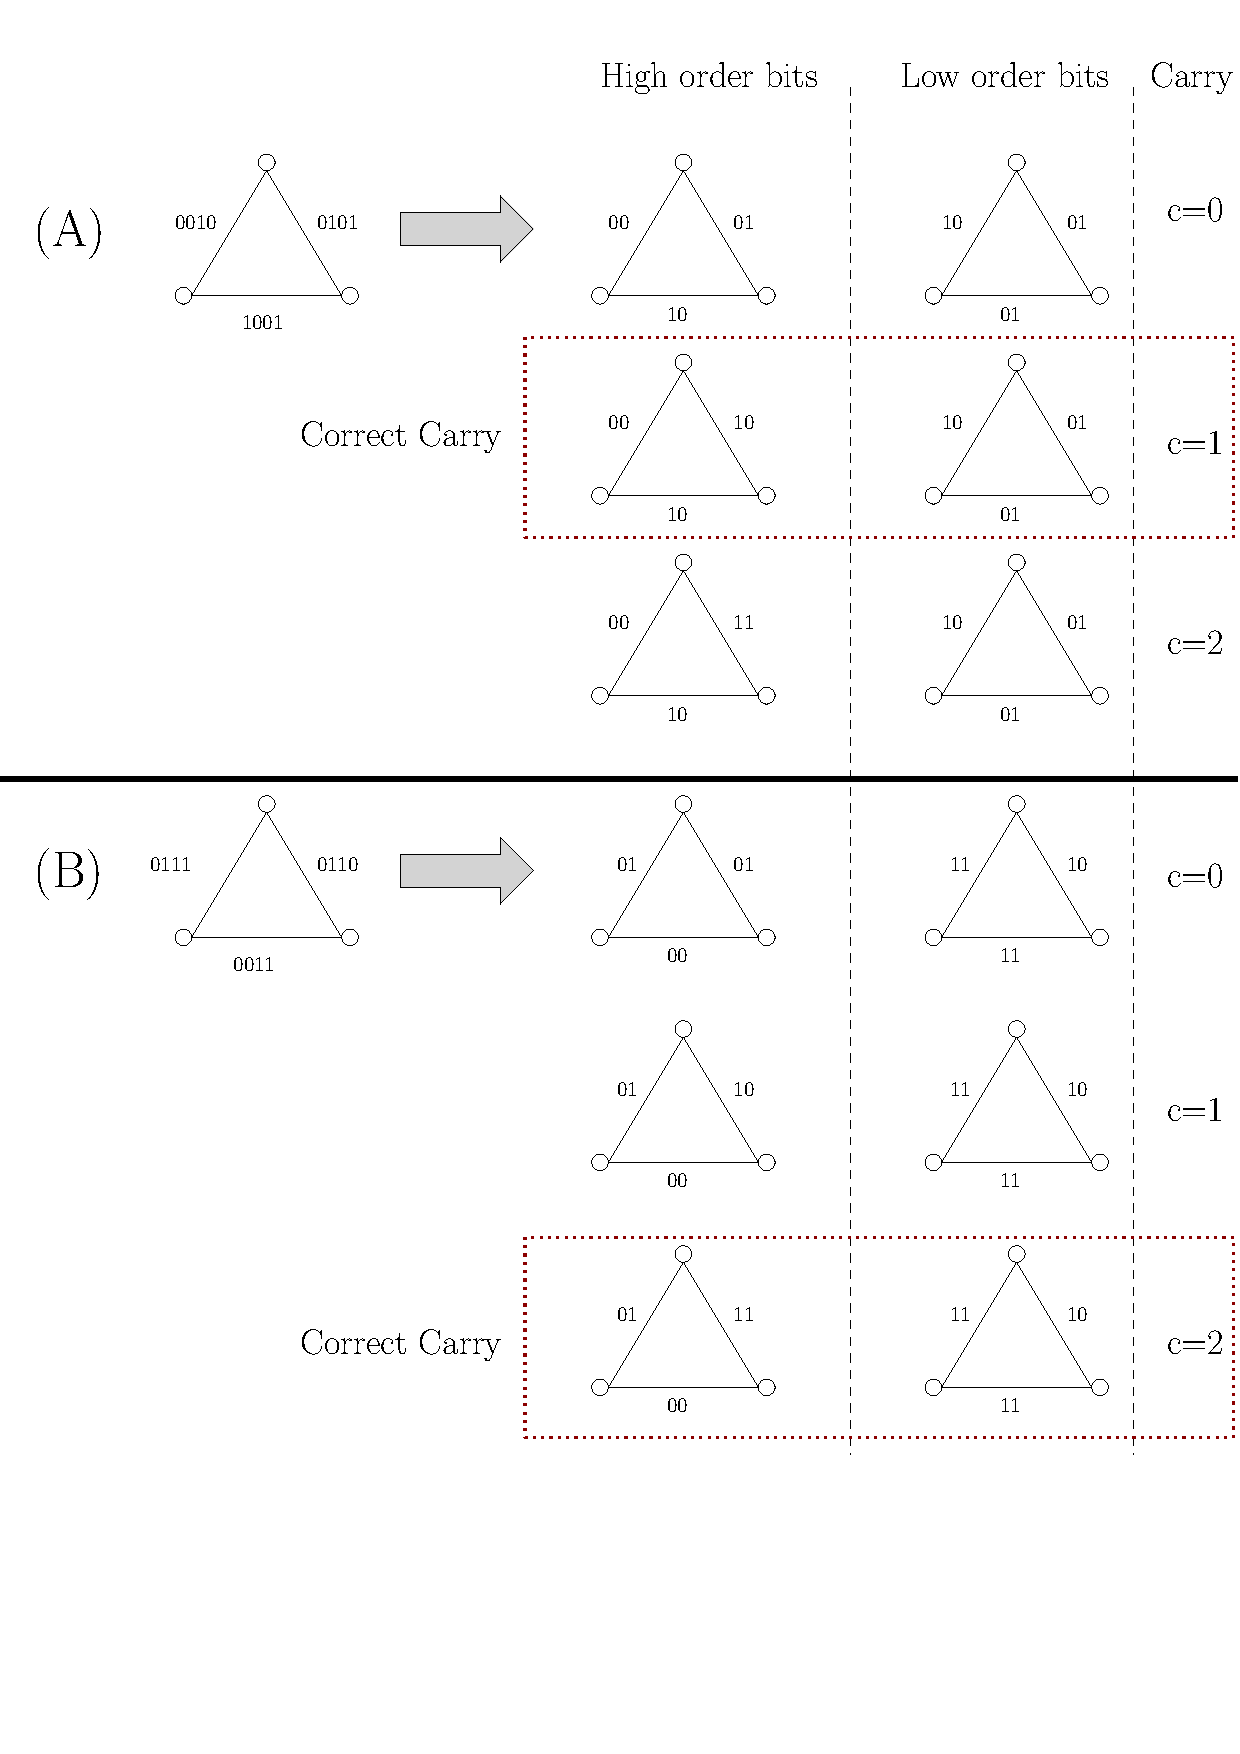
\includegraphics[scale=0.55]{fgcrypto/SplittableFig.pdf}
		\caption{An example of splitting the edges of triangles whose edges sum to $16$.}
		\label{fig:splittableRed}
	\end{figure}

	We will now show that we get the desired distributions in our list of instances depending on whether $I \sim D_0(\ZkC[R], n)$ or $I \sim D_1(\ZkC[R], n)$.
	\begin{itemize}
		\item $I \sim D_0(\ZkC[R], n)$. We need to show that every pair $(I_1^{(c)}, I_2^{(c)})$ is sampled from a distribution total variation distance $\le 2n^k/\sqrt R$ from $D_0(\ZkC[\sqrt R], n)^2$. Note that every pair is correlated very heavily with every other pair with respect to edge weights. But, within each pair, they are close to $D_0(\ZkC[\sqrt R], n)^2$.
		
		From lemma \ref{lem:TVDnosol}, this is TVD at most $\frac {n^k}{R}$ from just choosing edge-weights uniformly at random. So, consider $I' \sim \Generate(n,0)$, and do the same operations as for $I$ in the reduction: every bit in every edge weight will be chosen uniformly at random, meaning that the edge-weights in $\lowI'$ and $\highI'$ will also be uniform over $\sqrt R$. Permuting the nodes in $\lowI'$ does not change this distribution, and neither does adding (any) $c$ to a subset of edges in $\highI'$. Therefore, using lemma \ref{lem:TVDnosol}, \emph{both} $I_1'^{(c)}$ and $I_2'^{(c)}$ are TVD at most $\frac{n^k}{\sqrt R}$ from $D_0(\ZkC[\sqrt R], n)$. Since TVD is a metric, this implies that $I_1^{(c)}$ is TVD at most $n^k / \sqrt R$ from the distribution of $I_1'^{(c)}$, and thus at most $n^k / \sqrt R + n^k/ R$ from $D_0(\ZkC[\sqrt R], n)$ --- the same is true for $I_2^{(c)}$, even when conditioned on $I_1^{(c)}$. Therefore, the pair, for every $c$, is TVD at most $2(n^k / \sqrt R + n^k/ R) \le \frac{4 n^k}{\sqrt R}$.
		
		
		\item $I \sim D_1(\ZkC[R], n)$. We want to show that we get a list in which exactly one of the pairs of instances is distributed close to $D_1(\ZkC[\sqrt R], n)^2$.
		
		We will take a similar approach here, considering the planted distribution of $I$ instead of the true one. Let $I' \sim \Generate(n,1)$, so by lemma \ref{lem:TVDonesol}, $I'$ is TVD at most $2n^k/R$ from $D_1$. We will first show that $\lowI'$ is also drawn from a planted distribution over the range $\sqrt R$.
		Let $e'$ be the edge's weight that was changed to plant a zero clique. Now, for every edge except $e'_{low}$, the edges of $\lowI'$ are distributed uniformly. $e'$ is a randomly chosen edge corresponding to a randomly chosen clique in $I'$, and therefore $e'_{low}$ is also a randomly chosen edge corresponding to a randomly chosen clique in $\lowI'$. The act of making that clique sum to 0 mod $R$ also requires that the low-order bits sum to $0$ mod $\sqrt R$ --- otherwise the high-order bits cannot cancel out anything left over. Therefore, by setting $w(e')$ to the value making the clique sum to 0, we are exactly planting a clique in $\lowI'$. This distribution has TVD $\le \frac{2n^k}{\sqrt R}$ from $D_1(\ZkC[\sqrt R], n)$. Because $I_1'^{(c)}$ is just a permutation on the nodes of $\lowI'$ for every $c$, $I_1'^{(c)}$ will have TVD at most $\frac{2n^k}{\sqrt R}$ from $D_1$ as well.
		
		Now, we need that at least one of the pairs in this list to be close to $D_1(\ZkC[\sqrt R], n) \times D_1(\ZkC[\sqrt R], n) $. It will turn out that there exists a $c$ such that $I_2'^{(c)}$ will also be close to $D_1$ (whereas $I_1'^{(c)}$ is distributed close to $D_1$ for every $c$). Let $c^*$ be the correct carry --- that is for the clique planted in $I'$, $\sum_{e \in clique} \low w(e) = \sqrt R c^* \mod R$. Now, without loss of generality, we can assume that in the plant of $I'$, the edge $e^*$ chosen to complete the zero-$k$ clique was between partitions $P_i$ and $P_j$. So, considering every other edge in $I_2'^{(c^*)}$, it is distributed uniformly at random (adding $c^*$ will not change that distribution). Now, for that special clique $C^*$ that was planted in $I'$, we have that
		\begin{align*}
		\sum_{e \in C^*} w(e) &= \sqrt R \cdot \sum_{e \in C^*} \high w(e) + \sum_{e \in C^*} \low w(e)\\
		&= \sqrt R (\sum_{e \in C^*} \high w(e) + c^*)\\
		&= \sqrt R (\high w(e^*) + c^* + \sum_{e \in C^*, e \neq e^*} \high w(e)) = 0 \mod R
		\end{align*}
		Since the quantity $\sqrt R (\high w(e^*) + c^* + \sum_{e \in C^*, e \neq e^*} \high w(e))$ is 0 mod $R$, then $\high w(e^*) + c^* + \sum_{e \in C^*, e \neq e^*} \high w(e) = 0 \mod \sqrt R$.
		
		This means that $I_2'^{(c^*)}$ is drawn from $\Generate(n,1)$ over the range $\sqrt R$. Since TVD is a metric, we have that for $I \sim D_1(\ZkC[\sqrt R], n)$ (TVD at most $\frac {n^k}{R}$ from $\Generate(n, 1)$), there exists a $c^*$ such that $I_2^{(c^*)}$ is TVD at most $\frac{2n^k}{\sqrt R}$ from $D_1$ --- even when dependent on $I_1^{(c^*)}$. Therefore, the TVD of $(I_1^{(c^*)}, I_2^{(c^*)}) = \Split(I)$ to $D_1^2$ is at most $\frac{4 n^k}{\sqrt R}$.
	\end{itemize}
	Therefore, when $I \sim D_0(\ZkC[R], n)$, we get a list of pairs of instances TVD $\le 4n^k / \sqrt R$ from $D_0(\ZkC[R], n)^2$; the probability that any of these pairs here err is $\le(\binom k 2 + 1) \cdot \frac{4n^k}{\sqrt R}$ by a union bound. Similarly, when $I \sim D_1(\ZkC[R], n)$, we get there exists a pair in this list of the form $D_1(\ZkC[R], n)^2$; the probability of erring here is $\le \frac{4 n^k }{\sqrt R}.$
	
	Therefore, the total error here is $\le (\binom k 2 + 1) \cdot \frac{4n^k}{\sqrt R}$.
	\qed
\end{proof}

\paragraph{\zkclique~is Splittable Over Any Large Enough Range.}\label{sec:zkcsplittable}
Our techniques also generalize to any large enough range (even ones not of the form $4^x$). For example, if you believe that the problem is hard only over a prime range, we can prove that as well. As stated, our error is $\binom{k}{2}4^{\binom{k}{2}}3 n^k/\sqrt{R} = O(n^k/\sqrt R)$. For this to be meaningful, $R = \Omega(n^{2k})$, and in our constructions, $R$ is $\Omega(n^{6k})$. We will show in the next section why the zero $k$-clique problem is still hard over these larger ranges.

\begin{theorem}
	Zero-k-clique is generalized splittable over any range $R$, with error $\leq \binom{k}{2}4^{\binom{k}{2}}3 n^k/\sqrt{R}$. 
	\label{thm:zkcsplittable}
\end{theorem}
%TODO: go through that proof, too. is this statement correct?
\begin{proof}
	Given an instance $I$ with range $R$ we will produce $\leq \binom{k}{2}4^{\binom{k}{2}}$ instances, corresponding to guesses over what ranges the clique edge weights fall into. 
	
	Take the next smallest power $R' = \max\{2^{2x}| 2^{2x}<R \text{ and } x\in \mathbb{Z} \} $. 
	Now let $c = \lceil R/R' \rceil$. We will now create $c$ subsets of $R$ each of size $R'$.  $S_i = [R'i,R'(i+1)-1]$ for $i\in [0,c-2]$ and $S_{c-1} = [R-R' , R-1]$. Note that these subsets completely cover the range $[0, R-1]$ and are each of size $\le R'$. Let $\Delta_i = R'i$ for $i\in [0,c-2]$ and $\Delta_{c-1} = R-R'$. 
	
	Let the partitions of $I$ be $P_1, \ldots, P_k$. Let the set of edges between $P_i$ and $P_j$ be $E_{i,j}$. For all $i,j$ pairs $i\ne j$ we will choose a number between $[0,c-1]$. Call these numbers $g_{i,j}$ and the full list of them $\vec{g}$. For all possible choices of $\vec{g} \in \mathbb{Z}_{c}^{\binom{k}{2}}$ and $d \in [0, \binom{k}{2}-1]$ we will generate an instance $I_{\vec{g},d}$ over range $R'$ as follows: 
	
	For edge set $E_{i,j}$ that isn't $E_{1,2}$, for every edge in that edge set $e \in E_{i,j}$ if the weight of $e$, $w(e) \in S_{g_{i,j}}$ then set $w_{\vec{g},d}(e) = w(e) \mod R'$, if $w(e) \nin S_{g_{i,j}}$ then set $w_{\vec{g},d}$ to be a weight chosen uniformly at random from $[0, R'-1]$. Now note that these values are completely uniform over the range from $[0,R'-1]$. 
	
	For $E_{1,2}$ , for every edge in that edge set $e \in E_{1,2}$ if the weight of $e$, $w(e) \in S_{g_{1,2}}$ then set $w_{\vec{g},d}(e) = w(e) + dR \mod R'$, if $w(e) \nin S_{g_{1,2}}$ then set $w_{\vec{g}}$ to be a weight chosen uniformly at random from $[0, R'-1]$. Now note that these values are also completely uniform over the range from $[0,R'-1]$. 
	
	If no clique existed in the original instance then the chance that one is produced here is bounded by $n^k/R' \leq n^k4/R'$ by Lemma \ref{lem:TVDnosol}. Because we make so many queries this chance that any of them induce a clique is $\leq \binom{k}{2}4^{\binom{k}{2}}n^k4/R'$. 
	
	If the original instance was drawn from $D^{zkc}_{1}[R,n]$ then by Lemma \ref{lem:TVDonesol} this is only $\leq n^k/R + n^{k-2}/R$ total variation distance away from the instance generated by choosing each edge at random and then planting a clique. Then the procedure produces uniformly looking edges except for the planted edge. In the generated instance where the original zero clique edge weights are in $\vec{g}$ and the zero k-clique sums to $dR$ then the instance $I_{\vec{g},d}$ will have that planted edge set to the value such that zero k-clique from the original is a planted instance. So, that produced instance is drawn from a distribution with total variation distance $\leq n^k/R' + n^{k-2}/{R'}$ from $D^{zkc}_{1}[R',n]$. 
	
	Then we use the splitting procedure from Lemma \ref{lem:zkcSplitConvenientRange} to generate two instances from each of our generated instances. The probability of a no instance becoming a yes instance is $\leq \binom{k}{2}4^{\binom{k}{2}}3 n^k/\sqrt{R}$, if there is a yes instance then it will generate a yes instance and have total variation distance at most $\leq \binom{k}{2}4^{\binom{k}{2}}3 n^k/\sqrt{R}$ from $D^{zkc}_{1}[\sqrt{R'},n]^2$. \qed
\end{proof}
